%!TEX program = lualatex
\documentclass[tikz,border=8pt]{standalone}
\usepackage{fontspec}
\usepackage{unicode-math}
\usepackage{luamplib}
\usetikzlibrary{arrows.meta,decorations.pathmorphing}
\setmainfont{EBGaramond}[Extension=.otf, UprightFont=*-Regular, ItalicFont=*-Italic]
\setmathfont{Garamond-Math.otf}
\definecolor{paper}{HTML}{F4F0E8}
\definecolor{ink}{HTML}{2B241D}
\definecolor{green}{HTML}{5F7F67}
\pagecolor{paper}
\newsavebox{\orb}
\mplibforcehmode
\begin{document}
\begin{lrbox}{\orb}
\begin{mplibcode}
  input fiziko.mp;
  randomseed := 1729;
  defineMinStrokeWidth(0.14pt);
  defineLightDirection(-pi/6, pi/6);
  drawoptions(withcolor \mpcolor{green});
  beginfig(1);
    draw sphere.c(1.05cm);
  endfig;
\end{mplibcode}
\end{lrbox}
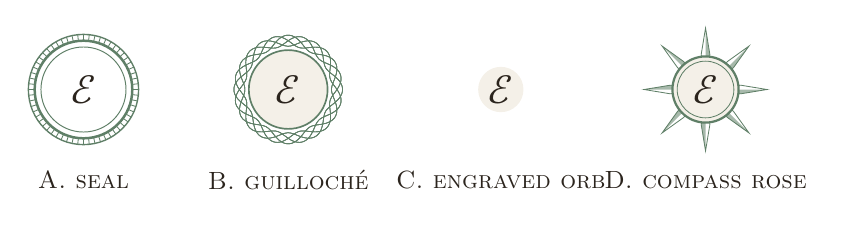
\begin{tikzpicture}[x=1cm,y=1cm, draw=ink, text=ink]
  % A: seal -- double ring + 60 fine ticks
  \begin{scope}[shift={(0,0)}]
    \draw[green, line width=.9pt] (0,0) circle (0.62);
    \draw[green, line width=.35pt] (0,0) circle (0.54);
    \foreach \a in {0,6,...,354} \draw[green, line width=.3pt] (\a:0.62) -- (\a:0.70);
    \draw[green, line width=.5pt] (0,0) circle (0.70);
    \node[font=\Large] at (0,0) {$\mathcal{E}$};
    \node[font=\small\scshape] at (0,-1.15) {A. seal};
  \end{scope}
  % B: guilloche rosette ring
  \begin{scope}[shift={(2.6,0)}]
    \foreach \k in {0,1,...,11}
      \draw[green, line width=.25pt, rotate=\k*15]
        plot[domain=0:360, samples=180, smooth] (\x:{0.62+0.07*cos(6*\x)});
    \fill[paper] (0,0) circle (0.5);
    \draw[green, line width=.6pt] (0,0) circle (0.5);
    \node[font=\Large] at (0,0) {$\mathcal{E}$};
    \node[font=\small\scshape] at (0,-1.15) {B. guilloché};
  \end{scope}
  % C: fiziko engraved sphere
  \begin{scope}[shift={(5.3,0)}]
    \node[inner sep=0] at (0,0) {\usebox{\orb}};
    \node[font=\Large, fill=paper, circle, inner sep=1pt] at (0,0) {$\mathcal{E}$};
    \node[font=\small\scshape] at (0,-1.15) {C. engraved orb};
  \end{scope}
  % D: compass rose star
  \begin{scope}[shift={(7.9,0)}]
    \foreach \a in {0,45,...,315} {
      \fill[green!55] (0,0) -- (\a-7:0.45) -- (\a:0.78) -- cycle;
      \draw[green, line width=.3pt] (0,0) -- (\a-7:0.45) -- (\a:0.78) -- (\a+7:0.45) -- cycle;
    }
    \fill[paper] (0,0) circle (0.42);
    \draw[green, line width=.8pt] (0,0) circle (0.42);
    \draw[green, line width=.3pt] (0,0) circle (0.36);
    \node[font=\Large] at (0,0) {$\mathcal{E}$};
    \node[font=\small\scshape] at (0,-1.15) {D. compass rose};
  \end{scope}
\end{tikzpicture}
\end{document}
